\documentclass{article}

\usepackage{../latex/styles/core} 

\bibliography{bibliography}

\title{Hardware Design Topics}
\author{Sai Mohan Kilambi}
\date{\today}
\begin{document}

\maketitle

\setcounter{tocdepth}{4}
\tableofcontents

\newpage

\section{Introduction}

This document contains notes on various hardware design topics that I find useful to take note of. We will cover hardware design elements, design patterns, static timing analysis, FPGA topics that are useful and other such things. 

\section{Register Types}
\subsection{Keeper Register}

A Keeper register latches the value in the current cycle and then holds in until a new update arrives and then it keeps that...so on and so forth. Note that it does not break a timing path. 

\begin{lstlisting}[style=svstyle]

module keeper_reg #(
	parameter type T = logic
) (
	input clk,
	input reset,
	
	input logic valid,
	input T sig_in,
	output T sig_out
);

	logic data;
	T data_reg;
	
	assign data = valid ? sig_in : data_reg;
	
	always_ff @(posedge clk) begin 
		data_reg <= data;
	end 
	
	assign sig_out = data;

endmodule

\end{lstlisting}

\begin{figure}[htbp]
    \centering
    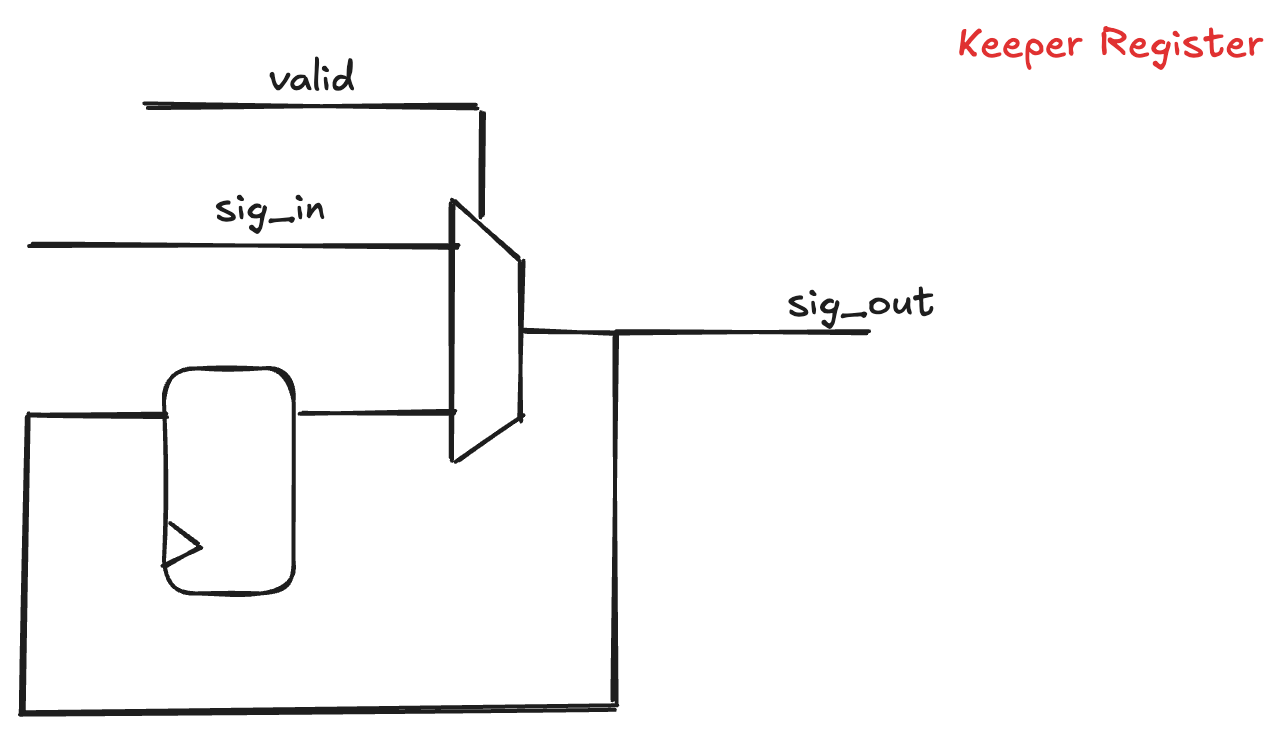
\includegraphics[width=0.4\textwidth]{./figs/keeper_reg.png}
    \caption{Keeper Reg}
    \label{fig:mylabel}
\end{figure}



\section{Race Conditions}
This section covers various cases of race conditions and how to handle them.
 
\subsection{When an update needs to be delayed until current transaction is done}
Sometimes we have a situation where an update comes in from another block or MMIO and the current block has a state-machine thats operating. If the state machine is in IDLE mode, we want to take the update in immediately. Otherwise we want to keep it pending until the current transaction is complete and then apply it. 

Lets say we have a block where
\begin{enumerate}
	\item An $update$ pulse is an input that moves a value from a holding register (that has been programmed via MMIO) into the active register. Lets call these $a\_holding\_reg$ and $a\_active\_reg$
	\item Lets say the block also has a state machine with the following states $IDLE$, $PROCESSING$.
\end{enumerate}

Here are the constraints
\begin{enumerate}
	\item If in $IDLE$ state, then update should reflect immediately.
	\item If not in $IDLE$ then wait for applying the change. 
\end{enumerate}

\begin{lstlisting}[style=svstyle]

logic transaction_in_progress;

// We say transaction is in progress when 
// 1. State is IDLE and a trigger shows up (this is an input probably into the block)
// 2. OR, we are in PROCESSING state. 
assign transaction_in_progress = trigger || state != IDLE; 

/*
In this code we track when update needs to be pending.
*/
always_comb begin 
	if ( trigger & transaction_in_progress ) begin 
		transaction_pending_next = 1;
	end else if ( transaction_pending & !transaction_in_progress ) begin
		transaction_pending_next = 0;
	end else 
		transaction_pending_next = transaction_pending;
end

`REG_RC ( transaction_pending, '0, transaction_pending_next )

// When should we do the update?
// 1) When we receive a trigger and we are not in the middle of a transaction
// 2) OR, we received a trigger in the middle of a transaction, we waited and now we are
//        clear to update.
assign do_update =  (trigger || transaction_pending) & (! transaction_in_progress);

// need to hold the data when we receive the trigger in the middle of a transaction
`REG_EC ( pending_reg, trigger & transaction_in_progress, a_holding_register)

// What is the source of the update?
assign source_data = (trigger & !transaction_in_progress) ? a_holding_reg : 
                     (transaction_pending & !transaction_in_progress) ? pending_reg :
                     a_active_reg;

`REG_EC ( a_active_reg, do_update, source_data )
					

\end{lstlisting}

\section{Common Hardware Blocks}
\subsection{Inferred Latch}

There are two kinds of memory elements in hardware design. One is a Flip-Flop and another is a Latch. A flip-flop changes its output state only on a rising or a falling edge of a clock. A latch on the other hand will change its state whenever its input changes state. However when input does not change state it will have to remember its previous output. 

In a case or if-else statement that is not complete, a latch may get inferred as shown in \ref{fig:inferred_latch}. This created a combination loop that cannot be timed. This is why inferred latches are harmful for ASIC/FPGA design. In the following code snippet, the comb\_out variable is not set when sel is $2'b11$. This will create a feedback. Always best to have complete case statement list or use \textit{unique case} statement.

\begin{Verbatim}
	
	logic [1:0] sel, comb_out;

	always_comb begin
		case(sel)
			2'b00: comb_out = 0;
			2'b01: comb_out = 1;
			2'b10: comb_out = 2; 
		endcase
	end
\end{Verbatim}


\subsection{Synchronous FIFO}


In a Sync FIFO the write and the read operate on the same clock. Let's break this down into its fundamental pieces. 
\begin{enumerate}
	\item Memory unit: This can be a bunch of registers of a certain width or BRAMs in an FPGA.
	\item Write Logic: This logic deals with keeping track of the write pointer. The write pointer indicates where the next data element should be written. 
	\item Read Logic: This portion deals with read pointer. The read pointer tracks the next location to be read.  
	\item Control and Status Logic: This portion keeps track of status signals such as EMPTY, FULL, ALMOST\_EMPTY, ALMOST\_FULL etc. COUNT signal will keep track of how many elements are currently present in the FIFO. 
\end{enumerate}

We will dig into each of these logic portions individually. 

\subsubsection{Count Logic}
Count keeps track of how many elements are currently in the FIFO. It has the following properties

\begin{enumerate}
	\item Should increment when there is a write but no read and its not full.
	\item Should decrement when there is a read but no write and its not empty.
	\item Should stay the same if there is no read OR write or there is a read AND write.
\end{enumerate}

\begin{Verbatim}
	always_ff @ (posedge clk) begin
		if ( ~resetn ) begin
			count <= '0;
		end else begin 
			count <= count_nxt;
		end 
	end	
	
	always_comb begin
		count_nxt = count;
		
		case ( {we, re} ) begin
			2'b10: count_nxt = count + 1;
			2'b01: count_nxt = count - 1;
		endcase
	end 
\end{Verbatim}


\subsubsection{Write Logic}

We first want to answer the following questions:
\begin{enumerate}
	\item When should a write occur? It should occur when the FIFO is not FULL. The FULL status signal should be used as a protection circuit for the writes. We can deal with this with valid, ready handshake on the write side. Valid is an input and ready should be high only if there is space in the FIFO. 
	\item Pointer logic: Write pointer should increment whenever there is a valid write transaction. Remember that it indicates where the next write should happen.
\end{enumerate}

\begin{Verbatim}
	// Write enable
	assign we = in_valid & in_ready;
	
	// Full Logic
	assign full = ~(count < SIZE); 	
	
	// In Ready Logic
	assign in_ready = !full;
	
	// Write pointer
	always_ff@ ( posedge clk ) begin 
		if (!resetn) begin
			wptr <= '0;
		end else begin
			if ( we )
				wptr <= f_incr_ptr ( wptr, SIZE );
		end
	end
	
	function addr_t f_incr_ptr(addr_t ptr, int SIZE);
		addr_t int_ptr;
		
		int_ptr = ptr < SIZE - 1 ? ptr+1 : 0;
	
		return int_ptr;
	endfunction;
	
	
	
\end{Verbatim}


\subsubsection{Read Logic}

We want to read when the down stream logic is ready to pop and when FIFO is not empty.

\begin{Verbatim}

	// Read Enable
	assign re = out_valid & out_ready;
	
	// Empty
	assign empty = count == 0;
	
	// Out Valid
	assign out_valid = !empty;
	
	// Read pointer
	always_ff@ ( posedge clk ) begin 
		if (!resetn) begin
			rptr <= '0;
		end else begin
			if ( re )
				rptr <= f_incr_ptr ( rptr, SIZE );
		end
	end
	
\end{Verbatim}

\subsubsection{Control and Status Logic}

We covered FULL, EMPTY and COUNT already. We only need ALMOST\_FULL and ALMOST\_EMPTY.

If we have given parameters for the count value for almost full and empty then we can just use this. By default, AMOST\_FULL\_SIZE is the same as SIZE and ALMOST\_EMPTY\_SIZE is same as 0.

\begin{Verbatim}
	assign alm_full = count >= ALMOST_FULL_SIZE;
	assign alm_empty = count <= ALMOST_EMPTY_SIZE;
\end{Verbatim}


\subsection{Ring Buffer or Queue}

Ring buffer is basically a queue. It is circular in that the read/write pointers wrap around. In strict definition, one should be able to overwrite old data in a ring-buffer but in our case we will handle empty/full conditions. Following is the contract for a ring buffer.
\begin{enumerate}
	\item An empty queue cannot be read from. That is, the output valid should be low if queue is empty.
	\item If a queue is full, then there should be back-pressure and new data cannot be written in.
\end{enumerate}




\printbibliography
	
\end{document}